\documentclass{beamer}
\usepackage[utf8]{inputenc}

\usetheme{Madrid}
\usecolortheme{default}
\usepackage{amsmath,amssymb,amsfonts,amsthm}
\usepackage{txfonts}
\usepackage{tkz-euclide}
\usepackage{listings}
\usepackage{adjustbox}
\usepackage{array}
\usepackage{tabularx}
\usepackage{gvv}
\usepackage{lmodern}
\usepackage{circuitikz}
\usepackage{tikz}
\usepackage{graphicx}

\setbeamertemplate{page number in head/foot}[totalframenumber]

\usepackage{tcolorbox}
\tcbuselibrary{minted,breakable,xparse,skins}



\definecolor{bg}{gray}{0.95}
\DeclareTCBListing{mintedbox}{O{}m!O{}}{%
  breakable=true,
  listing engine=minted,
  listing only,
  minted language=#2,
  minted style=default,
  minted options={%
    linenos,
    gobble=0,
    breaklines=true,
    breakafter=,,
    fontsize=\small,
    numbersep=8pt,
    #1},
  boxsep=0pt,
  left skip=0pt,
  right skip=0pt,
  left=25pt,
  right=0pt,
  top=3pt,
  bottom=3pt,
  arc=5pt,
  leftrule=0pt,
  rightrule=0pt,
  bottomrule=2pt,
  toprule=2pt,
  colback=bg,
  colframe=orange!70,
  enhanced,
  overlay={%
    \begin{tcbclipinterior}
    \fill[orange!20!white] (frame.south west) rectangle ([xshift=20pt]frame.north west);
    \end{tcbclipinterior}},
  #3,
}
\lstset{
    language=C,
    basicstyle=\ttfamily\small,
    keywordstyle=\color{blue},
    stringstyle=\color{orange},
    commentstyle=\color{green!60!black},
    numbers=left,
    numberstyle=\tiny\color{gray},
    breaklines=true,
    showstringspaces=false,
}
%------------------------------------------------------------
%This block of code defines the information to appear in the
%Title page
\title %optional
{1.2.19}
%\subtitle{A short story}

\author % (optional)
{Gautham-AI25BTECH11013}



\begin{document}


\frame{\titlepage}
\begin{frame}{Question}
In which quadrant or on which axis do each of the points $\brak{-2,4},\brak{3,-1},\brak{-1,0},\brak{1,2}$ and $\brak{-3,-5}$ lie?       Verify your answer by locating them on the Cartesian plane?
\end{frame}
\begin{frame}{Theoretical Solution}
If x=0 then the point $\brak{x,y}$ lies on y-axis.\\
If y=0 then the point $\brak{x,y}$ lies on x-axis.\\
If $x>0,y>0$ then the point $\brak{x,y}$ lies in $1^\text{st}$ quadrant.\\
If $x<0,y>0$ then the point $\brak{x,y}$ lies in $2^\text{nd}$ quadrant. \\
If $x<0,y<0$ then the point $\brak{x,y}$ lies in $3^\text{rd}$ quadrant. \\
If $x>0,y<0$ then the point $\brak{x,y}$ lies in $4^\text{th}$ quadrant. \\
\end{frame}
\begin{frame}{Theoretical Solution}
    We can infer that $\brak{-2,4}$ lies in $2^\text{nd}$ quadrant as $-2<0$,$4>0$. \\
Similarly $\brak{3,-1}$,$\brak{-1,0}$,$\brak{1,2}$,$\brak{-3,-5}$ lie on $4^\text{th}$quadrant,x-axis,$1^\text{st}$ quadrant,$3^\text{rd}$ quadrant respectively . 
\end{frame}
\begin{frame}[fragile]
\frametitle{C Code}
   \begin{lstlisting}
#include <stdio.h>

const char* check_quadrant(int x, int y) {
    if (x == 0 && y == 0) {
        return "Origin";
    } else if (x == 0) {
        return "Y-axis";
    } else if (y == 0) {
        return "X-axis";
    } else if (x > 0 && y > 0) {
        return "Quadrant I";
    } else if (x < 0 && y > 0) {
        return "Quadrant II";
    } else if (x < 0 && y < 0) {
        return "Quadrant III";
    } else {
        return "Quadrant IV";
    }
}
   \end{lstlisting}
\end{frame}
\begin{frame}[fragile]
\frametitle{Python-C Code}
   \begin{lstlisting}
 import numpy as np
import matplotlib.pyplot as plt
import ctypes

# Load the compiled library
quadrant_check = ctypes.CDLL('./func.so')
quadrant_check.check_quadrant.argtypes = [ctypes.c_double, ctypes.c_double]
quadrant_check.check_quadrant.restype = ctypes.c_char_p
   \end{lstlisting}
\end{frame}
\begin{frame}[fragile]
\frametitle{Python-C Code}
   \begin{lstlisting}
   def main():
    # Define the points ONCE
    points = [(-2, 4), (3, -1), (-1, 0),(1, 2), (-3, -5)]
    
    # Check each point using the C function
    print("Point Locations:")
    print("=" * 40)
    
    for i, (x, y) in enumerate(points):
        result_bytes = quadrant_check.check_quadrant(x, y)
        result = result_bytes.decode('utf-8')
        print(f"Point {i+1}: ({x}, {y}) -> {result}")
    print("=" * 40)
   \end{lstlisting}
\end{frame}
\begin{frame}[fragile]
\frametitle{Python-C Code}
   \begin{lstlisting}
   plt.figure(figsize=(8, 8))
    plt.axhline(0, color='black')  # x-axis
    plt.axvline(0, color='black')  # y-axis

    for (x, y) in points:
        plt.scatter(x, y, s=80)
        plt.text(x+0.1, y+0.1, f"({x},{y})", fontsize=9)

    plt.title("Points on Cartesian Plane (Q1.2.19)")
    plt.xlabel("X-axis")
    plt.ylabel("Y-axis")
    plt.grid(True)
    plt.gca().set_aspect('equal', adjustable='box')
    plt.savefig("/home/gauthamp/ee1030-2025/ai25btech11013/matgeo/1.2.19/figs/plotc.png")
    plt.show()

   \end{lstlisting}
\end{frame}
\begin{frame}[fragile]
\frametitle{Python Code}
   \begin{lstlisting}
import matplotlib.pyplot as plt

# Given points
points = [(-2, 4), (3, -1), (-1, 0), (1, 2), (-3, -5)]


# Plotting using plt only
plt.axhline(0, color='black')  # x-axis
plt.axvline(0, color='black')  # y-axis

for (x, y) in points:
    plt.scatter(x, y, s=80)
    plt.text(x+0.1, y+0.1, f"({x},{y})", fontsize=9)
\end{lstlisting}
\end{frame}
\begin{frame}[fragile]
\frametitle{Python Code}
   \begin{lstlisting}
plt.title("Points on Cartesian Plane (Q1.2.19)")
plt.xlabel("X-axis")
plt.ylabel("Y-axis")
plt.grid(True)
plt.gca().set_aspect('equal', adjustable='box')
plt.savefig("/home/gauthamp/ee1030-2025/ai25btech11013/matgeo/1.2.19/figs/Figure1.png")
plt.show()
\end{lstlisting}
\end{frame}
\begin{frame}{Plot}
    \begin{figure}[h!]
    \centering
    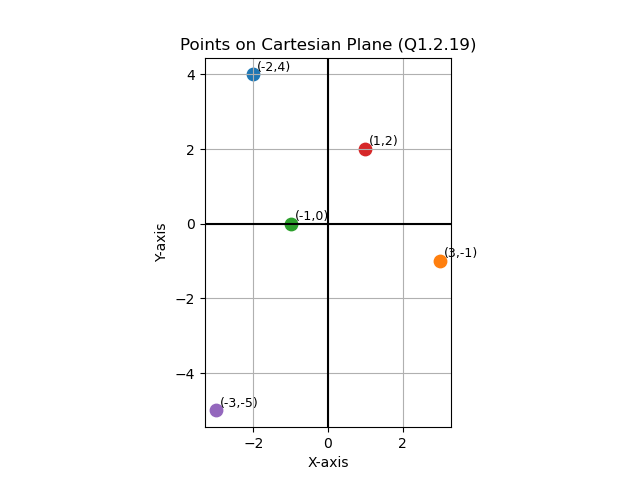
\includegraphics[height=0.6\textheight, keepaspectratio]{figs/Figure1.png}
    \label{figure_1}
\end{figure}
\end{frame}

\end{document}
